\documentclass{article}
\usepackage{preamble}

\begin{document}
\pagecolor{black!83}
\color{black!5}
\begin{center}
	\texttt{work-done by a variable force}
\end{center}
\vspace*{\fill}
\begin{center}
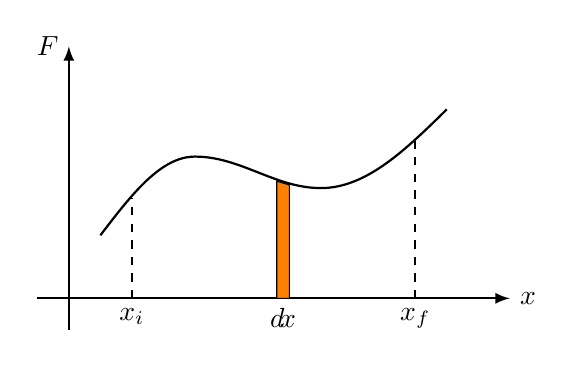
\begin{tikzpicture}[thick, scale=0.8]
	\draw[-latex] (-0.5, 0)--(7, 0) node[right]{$x$};
	\draw[-latex] (0, -0.5)--(0, 4) node[left]{$F$};
	\draw[smooth, ] (0.5, 1) sin(2, 2.25) cos(3, 2) sin(4, 1.75) cos (6, 3);
	\draw[dashed] (1, 0) node[below]{$x_i$} --(1, 1.6);
	\draw[dashed] (5.5, 0) node[below]{$x_f$}--(5.5, 2.5);
	\draw[thin, fill=orange] (3.3, 0)--(3.3, 1.86)--(3.5, 1.8)--(3.5, 0)--cycle;
	\node at (3.4,0)[below]{$d\!x$};
	
\end{tikzpicture}
\end{center}
\begin{align*}
W &= \int_{\vec{r}_i}^{\vec{r}_f} \vec{F} \cdot d\vec{r} \\[4 mm]
W &= \int_{x_i}^{x_f} F_x \; d\!x + \int_{y_i}^{y_f} F_y \; d\!y + \int_{z_i}^{z_f} F_z \; d\!z 
\end{align*}


\vspace*{\fill}
\end{document}